\chapter{Angular}\label{angular}

\section{Introduzione}

Lo scopo della pagina web prodotta in Angular , e' quello di fornire le operazioni necessarie per attuare la modifica dello stato della lampada , sfruttando le funzionalita' dell'API. \\
Nell'ottica del poc , la modifica e' riservata alla lampada con id = 1 . \\
L'utente ha la capacita' di visualizzare lo stato corrente della lampada, sia in forma visiva che testuale, e modificarne lo stato. 

\section{Funzionamento}

\subsection{lamp-button.component.ts}
Questo componente consiste in un pulsante che cambia lo stato di una lampada. Visualizza inoltre un'immagine della lampada , variabile in base allo stato, e il suo stato corrente scritto in forma testuale.

\subsection{All'avvio della pagina - OnInit()}
All'avvio della pagina web,viene chiamato il metodo getStatus().\\
Il metodo getStatus() è responsabile di ottenere lo stato corrente della lampada tramite una chiamata GET, ed aggiornare il valore locale nel BehaviorSubject lampStatus\$ con il nuovo stato.

\subsection{getStatus()}
Questo metodo recupera lo stato corrente della lampada attraverso una chiamata GET all'endpoint (/lamps/1). \\

\subsection{Al tocco della lampada - toggleLamp()}

Si offre il metodo toggleLamp(), tale metodo cambia lo stato della lampada tramite una chiamata PUT , da un valore locale "On" , ad "Off" , e viceversa.

\section{template HTML}
Il template HTML mostra un'immagine della lampada e il suo stato corrente. \\
Tale immagine e' anche un pulsante che chiama il metodo toggleLamp(), quando viene cliccato.

\section{Metodi di supporto}

\subsection{getData\$()}
Si offre il metodo getData\$(), il quale effettua una richiesta HTTP GET all'endpoint API per recuperare lo stato corrente della lampada.

\subsection{toggleLamp\$()}
Questo metodo effettua una richiesta HTTP PUT all'endpoint API per cambiare lo stato della lampada. \\
Prende un parametro "status" che rappresenta lo stato corrente della lampada. \\
Se lo stato è "On", invia una modifica del parametro in "Off" per spegnere la lampada, e viceversa.

\section{immagini}

\begin{figure}[H]
    \centering
    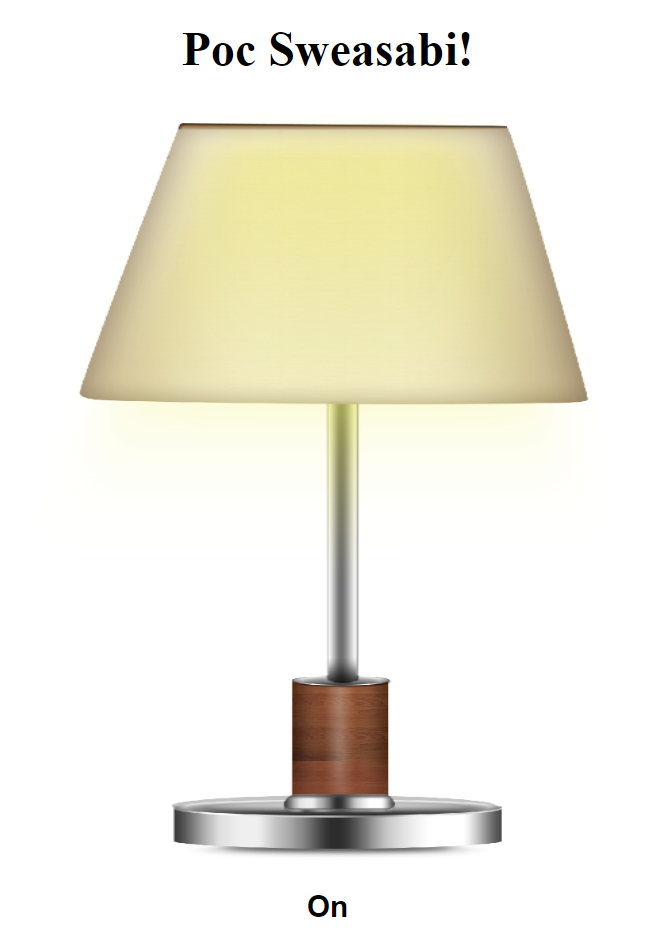
\includegraphics[width=\linewidth]{getlamps.png}
    \caption{Button fa richiesta di stato iniziale su /Lamps}
\end{figure}


\begin{figure}[H]
    \centering
    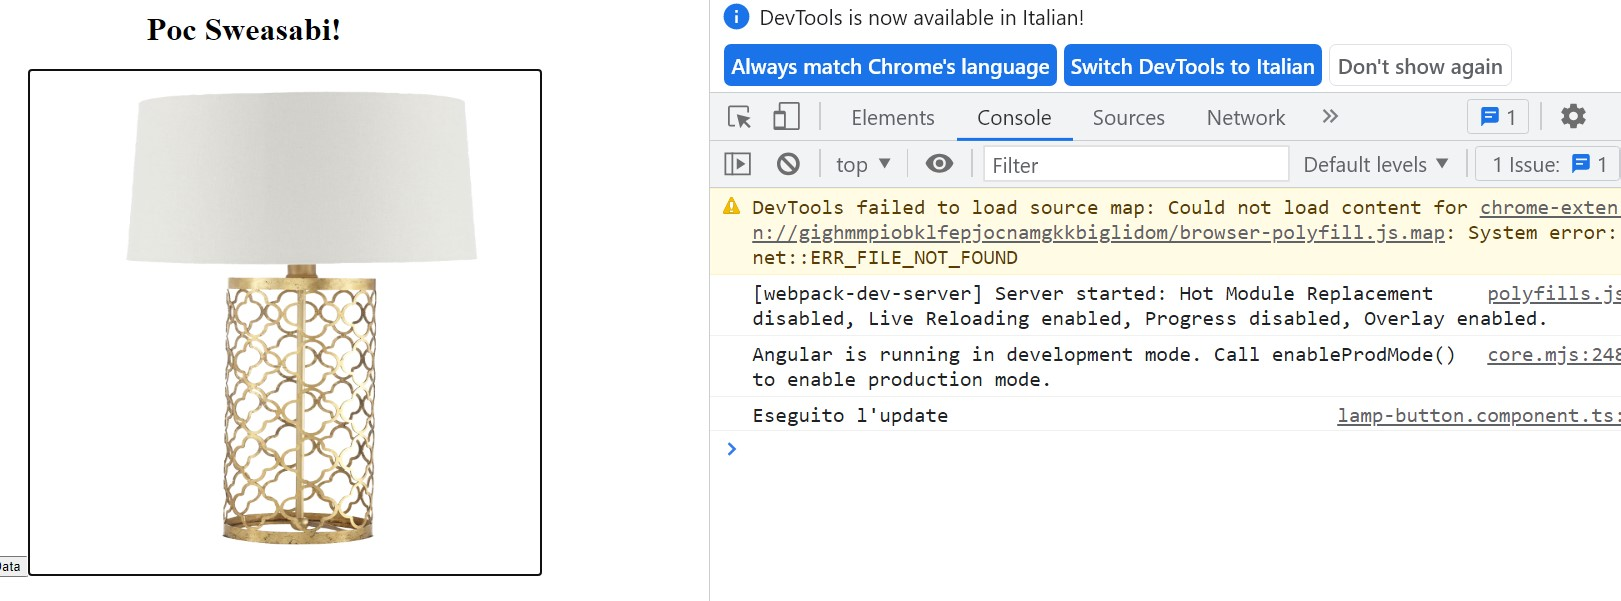
\includegraphics[width=\linewidth]{modifylamps.jpg}
    \caption{Button fa cambio di stato su /Lamps/1}
\end{figure}

\begin{figure}[H]
    \centering
    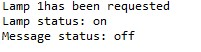
\includegraphics[width=0.3\linewidth]{modifylamps2.png}
    \caption{Button fa cambio di stato su /Lamps/1}
\end{figure}
